%   Filename    : chapter_4.tex 
\chapter{Research Methodology}
This chapter lists and discusses the specific steps and activities that were performed  to accomplish the project. 
The discussion covers the activities from pre-proposal to Final SP Writing.

\section{Research Activities}
This project aimed to create an automated attendance system with the help of RFID together with facial recognition technology. This attendance system was designed to replace and reduce the usage of manual attendance such as the written and oral and enhance its lacking optimized features such as security, reliability, authenticity, and integrity using the student’s RFID and facial biometric.

The system functioned by tapping the RFID of the students with real time facial capture through face recognition technology. The identity of the students was verified through the unique serial number of their RFID that matches from the system database while the face recognition served as the two-factor authentication. The face recognition worked by capturing the students face then matched through the system database. The attendance is only validated once both student’s unique serial number in their RFID and their face has been verified.

To make the system functional, several data from the students need to be collected. Those are the student’s name, student number, student’s unique serial number of  their RFID, and their facial biometrics. These data gathered either online or face to face. Students are encouraged to download any of the RFID card readers to know their RFID’s serial number but in case they are incapable of doing that. Face to is an option where we can provide a physical RFID card reader. The facial recognition data were gathered through capturing their cropped image to be more accurate. 

The hardware components used in this system are:
RFID scanner: Which was used to read the RFID given to the students. This is also responsible for taking the students unique serial number on their RFID ensuring the integrity of the students.
USB connector: This was used to connect the RFID scanner to the Laptop or Raspberry Pi. Flex cable: This was used to connect the Raspberry Pi Vision Camera to Raspberry Pi.
Laptop / Raspberry Pi: This served as the main processing unit. The laptop or raspberry pi was used for running the required algorithm to make the face recognition and read the RFID correctly. Overall, the laptop / raspberry pi was in charge of handling the data.
Raspberry Pi Vision Camera: Captured the student’s facial image while scanning the RFID to the RFID scanner. 

\section{RFID and Face Recognition}
We use the UP RFID for our system. This approach enhances security by combining something you have (the RFID token) with something you are (your face).
\subsection{RFID as a Token}
The RFID token (the UP RFID) provides a unique identifier (ID) for the user. The RFID reader scans the token and extracts the unique ID. This ID is used to retrieve the corresponding user profile from a database.
\subsection{Face Recognition as a Verifier}
Face recognition ensures that the person presenting the RFID token is the authorized user associated with that token.

\section{Face Recognition}
Face recognition pipeline can be simplified into 2 steps:
\begin{enumerate}
	\item Face Detection: The process of finding the faces in a viewfinder and draw bounding boxes around the detected face. A pretrained YOLOv8n model was used as the base model for face detection. The resulting cropped image was feed into the face recognition model. It runs on the IMX500 chip in the Raspberry Pi AI Camera for inference, freeing the CPU for other task \cite{sony_imx500}. As on now, only YoloV8 officially supports exporting their model to the Rasperberry Pi AI camera \cite{ultralytics_imx500}. For this to work seamlessly, it is recommended to avoid low-light conditions. According to Zhou (2025), images captured in low-light conditions tend to be of poor quality, are easily disrupted by background noise, and suffer loss of detail, which lowers the accuracy of facial verification in the next step.
	
	\item Face verification: The task of comparing 2 faces and checking if they are of the same identity. The model we chose for this is MobileFaceNet which is a face recognition model optimized for mobile and embedded devices like the Raspberry Pi \cite{chen2018mobilefacenets}.
\end{enumerate}

\subsection{YoloV8n for Face Detection}

We selected the YOLOv8n model for face detection due to its compatibility with the Raspberry Pi AI Camera and its efficiency for edge inference. This model was fine-tuned on a dataset of over 10,000 face images and trained for 100 epochs using a batch size of 16 on a single NVIDIA V100 16GB GPU. It achieved the following metrics:

\begin{itemize}
	\item \textbf{Precision (IoU $\geq$ 0.5):} 77.2\%
	\item \textbf{Recall (IoU $\geq$ 0.5):} 48.9\%
	\item \textbf{mAP@50:} 55.98\%
	\item \textbf{mAP@50--95:} 29.05\%
\end{itemize}

These results demonstrate that the model has strong face detection capabilities, with a good balance between precision and recall. Figure~\ref{fig:yolo-metrics} presents the performance curves for all four metrics across training epochs.

\begin{figure}[H]
	\centering
	\begin{subfigure}[b]{0.48\textwidth}
		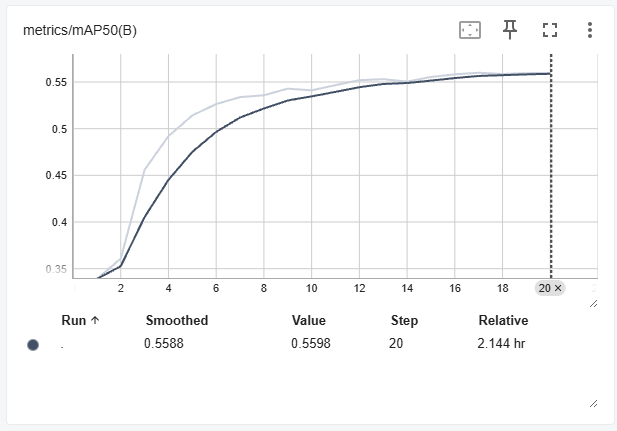
\includegraphics[width=\textwidth]{figures/chapter4/map50.png}
		\caption{mAP@50}
	\end{subfigure}
	\hfill
	\begin{subfigure}[b]{0.48\textwidth}
		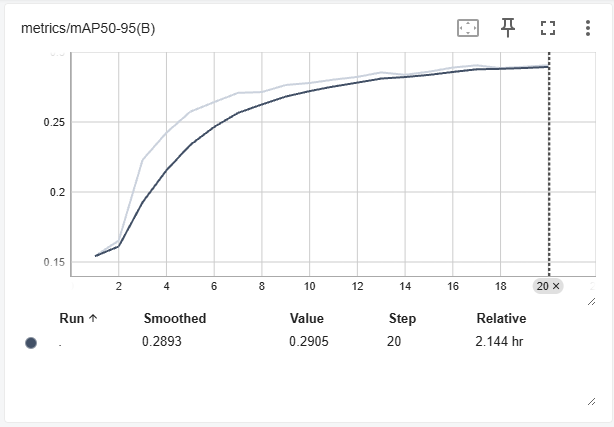
\includegraphics[width=\textwidth]{figures/chapter4/map5095.png}
		\caption{mAP@50--95}
	\end{subfigure}
	
	\vspace{1em}
	
	\begin{subfigure}[b]{0.48\textwidth}
		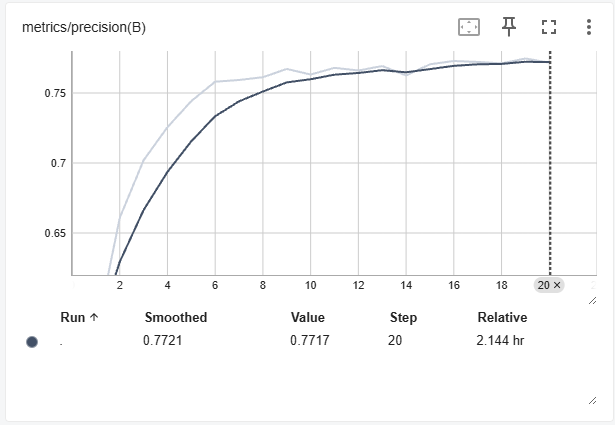
\includegraphics[width=\textwidth]{figures/chapter4/precision.png}
		\caption{Precision (IoU $\geq$ 0.5)}
	\end{subfigure}
	\hfill
	\begin{subfigure}[b]{0.48\textwidth}
		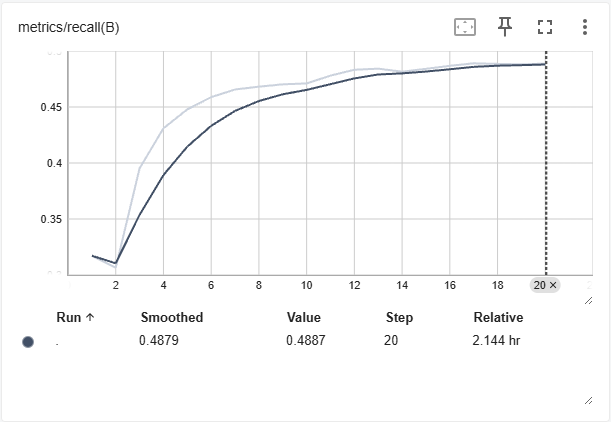
\includegraphics[width=\textwidth]{figures/chapter4/recall.png}
		\caption{Recall (IoU $\geq$ 0.5)}
	\end{subfigure}
	
	\caption{Performance metrics of the YOLOv8n face detection model across training epochs.}
	\label{fig:yolo-metrics}
\end{figure}

The YOLOv8n model was selected primarily for its support by the Ultralytics framework, which enables easy conversion and compression using Sony's Model Compression Toolkit. The model was compressed from its original 6MB size to around 3MB, fitting within the 8MB memory constraint of the Sony IMX500 chip. This allowed real-time face detection to be performed directly on the camera hardware, offloading the computation from the Raspberry Pi 5 CPU and improving overall system responsiveness.

\subsection{MobileFaceNet for Face Verification}

For the face verification task, we utilized the pretrained MobileFaceNet model due to its small size (863KB) and optimization for real-time inference on mobile and embedded devices. The model outputs a feature embedding for each 112$\times$112 facial image. Verification is performed using cosine similarity between embeddings.

We tested the discriminative ability of the model using the Labeled Faces in the Wild (LFW) Dataset via sklearn. The dataset includes 13,233 images of 5,749 people. The sklearn package provides a 300 pairs of same + 300 pairs of different people per fold. We tested the model in 10 folds:

\begin{itemize}
	\item \textbf{AUC (Area Under ROC Curve):} 0.77
	\item \textbf{Accuracy (at threshold 0.60):} 68.6\%
\end{itemize}

While the model sacrifices some performance for speed due to compression to TensorFlow Lite format, its accuracy and verification speed remain suitable for our use case. This trade-off was necessary for reliable inference on the Raspberry Pi 5 hardware within the system’s real-time constraints.

Compared to models of hundreds of MB in size, the performance of the model is good but can be better. Figure \ref{fig:roc_curve} shows the ROC AUC of the model of 0.77. An Area Under the Curve (AUC) of 0.77 means that if we pick one genuine (same‐person) pair and one impostor (different‐person) pair at random, there’s a 77\% chance the model will score the genuine pair higher.
\begin{figure}[h] % 'h' places the figure approximately here in the text
	\centering
	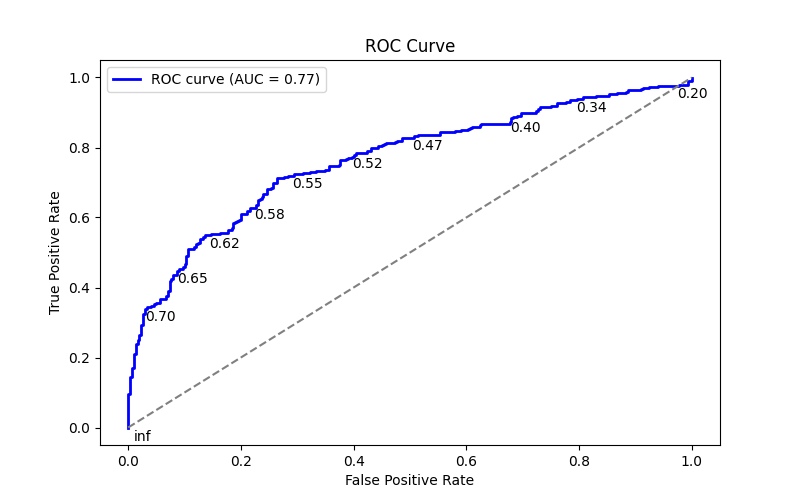
\includegraphics[width=1\textwidth]{figures/chapter4/roc_curve.png} % Adjust width as needed
	\caption{Receiver Operating Characteristic (ROC) Curve for Face Verification}
	\label{fig:roc_curve}
\end{figure}

\clearpage
Next, we evaluate the model's overall accuracy using the chosen threshold. As shown in Figure \ref{fig:fixed_thresh}, the confusion matrix corresponds to a fixed threshold of 0.6. This threshold was selected to strike a practical balance between security (minimizing false positives) and reliability (maintaining acceptable true positive rates). At this setting, the model achieved an average accuracy of 68.6\% across ten cross-validation folds. While this accuracy may not appear high, it is important to note that the evaluated model is a TensorFlow Lite version, optimized and compressed for real-time inference on a Raspberry Pi 5. This compression trades off some performance for significantly improved inference speed on edge devices.
\begin{figure}[h] % 'h' places the figure approximately here in the text
	\centering
	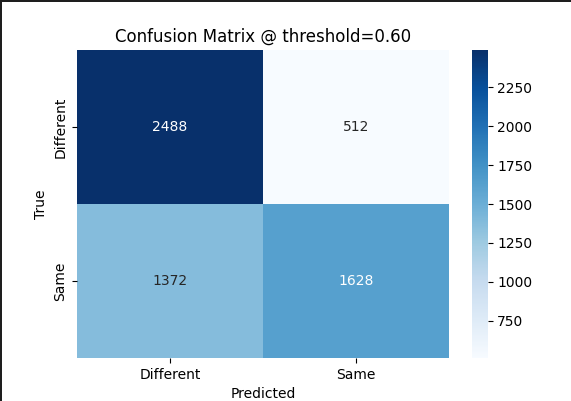
\includegraphics[width=0.75\textwidth]{figures/chapter4/fixed_thresh_matrix.png} % Adjust width as needed
	\caption{Confusion Matrix at a Threshold of 0.60}
	\label{fig:fixed_thresh}
\end{figure}

\section{Hardware Development Tools}
Our current prototype uses hardware components that are commonly used in the industry to build an integrated system. All of the tools are readily available. These include but are not limited to:

\begin{itemize}
	\item	RFID Scanner - Used as a reader for the RFID. The RFID scanner allows us to have secured and efficient way of identifying the student's unique serial number.
	
\end{itemize}

\begin{itemize}
	\item	Raspberry Pi AI Camera - The newly released camera module for Raspberry Pi hardware that allows us to capture the student's facial image while scanning the RFID with the use of RFID scanner. It uses an embedded AI accelerator for efficient processing of face data.
	
\end{itemize} 

\begin{itemize}
	\item	Raspberry Pi - Serves as the main processing unit which allows us to integrate the other hardware together with the necessary software.
	
\end{itemize}

\begin{itemize}
	\item	USB Connector -  Serves as connector for the RFID scanner and Raspberry Pi.
	
\end{itemize}

\begin{itemize}
	\item	Flex Cable -  Serves as connector for the Raspberry Pi Vision Camera and Raspberry Pi. 
	
\end{itemize}

\section{Software Development Tools}
\label{sec:devtools}
Our current protoype include these frameworks and tools that are heavily used in the industry for rapid development and deployment of web applications. All of the tools used are open source. These include but are not limited to:

\begin{itemize}
	\item	Django - The web framework for perfectionists with deadlines. Django, which serves as the backend server, allows us to interface with the database server to do queries in the Python using Django's Object Relational Mapping tool(ORM). We can easily integrate popular pretrained facial recognition models as they are typically written in Python.
\end{itemize}

\begin{itemize}
	\item	Django Ninja - Creates the REST API on top of our Django backend to allow the frontend to consume the backend content.
\end{itemize}

\begin{itemize}
	\item	NuxtJS - The frontend JavaScript framework used to build our web interface. Includes all the tools for routing, quering, and security. By default, it renders our web interface in Server Side Rendering(SSR) mode. Most of the work happens in the server and no authentication tokens are stored in the client browser. This increases security since authentication tokens are only added in the server side per request.
\end{itemize}

